\documentclass[10pt,aspectratio=169]{beamer}
\usepackage[utf8]{inputenc}
\usepackage[T1]{fontenc}
\usepackage[spanish]{babel}
\usepackage{lmodern}
\usepackage{amsmath,amssymb}
\usepackage{booktabs}
\usepackage{graphicx}
\usepackage{xcolor}

% Tema sobrio
\usetheme{metropolis}
\metroset{
  block=fill,
  progressbar=frametitle,
  numbering=fraction,
  sectionpage=progressbar,
}
\setbeamercolor{progress bar}{fg=blue!60!black}
\setbeamercolor{frametitle}{bg=blue!70!black}

\title{Optimizaci\'on espacial de Needleman--Wunsch \\
       y filogenia molecular del citocromo c}
\subtitle{Examen Parcial -- CC0F3 Biolog\'ia Computacional}
\author{Franklin Espinoza Pari \\ \small 20210135D}
\institute{Universidad Nacional de Ingenier\'ia}
\date{Mayo de 2026}

\begin{document}

\maketitle

% ---------------------------------------------------------------
\section{Contexto: PC2 \(\to\) Parcial}

\begin{frame}{De d\'onde partimos}
\textbf{Base PC2:} Needleman--Wunsch (global) + Smith--Waterman (local) en Python OO con \emph{Template Method} y \emph{Strategy}; matrices SIMPLE, PAM y BLOSUM.

\bigskip
\textbf{Dos preguntas del parcial}, resueltas reutilizando esa base:

\begin{itemize}
  \item \textbf{Proyecto 1.} El l\'imite pr\'actico de NW es la \emph{memoria}: $O(mn)$.
        $\Rightarrow$ \textbf{algoritmo de Hirschberg} para llegar a $O(\min(m,n))$.
  \item \textbf{Proyecto 2.} Distancia evolutiva por pares con NW $\Rightarrow$
        \textbf{matriz de distancias y dendrograma} para 6 ort\'ologos de citocromo c.
\end{itemize}

\bigskip
\textbf{Datos reales} (NCBI/UniProt, no inventados): CDS de \texttt{CYCS} humano/rat\'on y prote\'inas citocromo c de Humano, Chimpanc\'e, Gorila, Rat\'on, Gallina, At\'un.
\end{frame}

% ---------------------------------------------------------------
\section{Proyecto 1: Hirschberg}

\begin{frame}{El problema de memoria de NW}
La recurrencia
\[
H_{i,j} = \max\!\left\{H_{i-1,j-1}+s(\sigma_1[i],\sigma_2[j]),\; H_{i-1,j}+g,\; H_{i,j-1}+g\right\}
\]
solo depende de la fila anterior $\Rightarrow$ el \textbf{score} cabe en $O(n)$ (dos filas).

\medskip
\textbf{Pero el traceback necesita la matriz completa.} Para un cromosoma de $10^5{\times}10^5$ celdas eso son $\sim 40$~GiB en enteros de 32~bits: inviable.

\bigskip
\begin{block}{Idea de Hirschberg (1975)}
Divide-and-conquer: parte $\sigma_1$ por la mitad $i^* = m/2$ y busca $j^*$ tal que
$j^* = \arg\max_j\bigl(F[j] + B[n-j]\bigr)$, con $F, B$ calculados en $O(n)$ memoria.
Recurre sobre las dos mitades y concatena. \textbf{Tiempo $O(mn)$, memoria $O(\min(m,n))$.}
\end{block}
\end{frame}

\begin{frame}{Implementaci\'on sobre la jerarqu\'ia de la PC2}
Tres archivos nuevos, \textbf{cero modificaciones} a la PC2 (Open/Closed):

\begin{itemize}
  \item \texttt{parcial/nw\_two\_rows.py} -- primitiva $O(n)$ que devuelve la \emph{\'ultima fila} de NW.
  \item \texttt{parcial/hirschberg.py} -- clase \texttt{HirschbergAligner} con la misma interfaz \texttt{align()} que \texttt{NeedlemanWunsch}.
  \item \texttt{parcial/benchmark.py} -- medici\'on de tiempo y memoria pico con \texttt{memory\_profiler}.
\end{itemize}

\medskip
\textbf{Validaci\'on de correcci\'on (CDS humano vs rat\'on, 318 bases):}
\begin{center}
\begin{tabular}{lccc}
\toprule
 & score & longitud & identidad \\
\midrule
NW cl\'asico  & 260 & 320 & 90.6\,\% \\
Hirschberg   & 260 & 320 & 90.6\,\% \\
\bottomrule
\end{tabular}
\end{center}

\smallskip
\small\emph{Score id\'entico; la cadena exacta puede diferir en empates de traceback (varios alineamientos \'optimos).}
\end{frame}

\begin{frame}{Benchmark: tiempo y memoria}
\begin{columns}[T]
\column{0.5\textwidth}
\centering
\small
\begin{tabular}{rrrr}
\toprule
$L$ & $t_{\text{NW}}$ & $\Delta m_{\text{NW}}$ & $\Delta m_{\text{HB}}$ \\
(bases) & (ms) & (MiB) & (MiB) \\
\midrule
200  & 52    & 2.0    & 0.0 \\
400  & 55    & 2.1    & 0.0 \\
800  & 155   & 15.7   & 0.0 \\
1600 & 585   & 78.8   & 0.0 \\
3200 & 2322  & 357.6  & 0.0 \\
6400 & 9274  & \textbf{1429.7} & \textbf{0.0} \\
\bottomrule
\end{tabular}

\medskip
NW $\to$ \textbf{1.4 GiB} para 6400 bases.\\
Hirschberg $\to$ baseline (0 MiB delta).\\
\smallskip
Tiempo: HB es $\sim 2.5\times$ m\'as lento.

\column{0.5\textwidth}
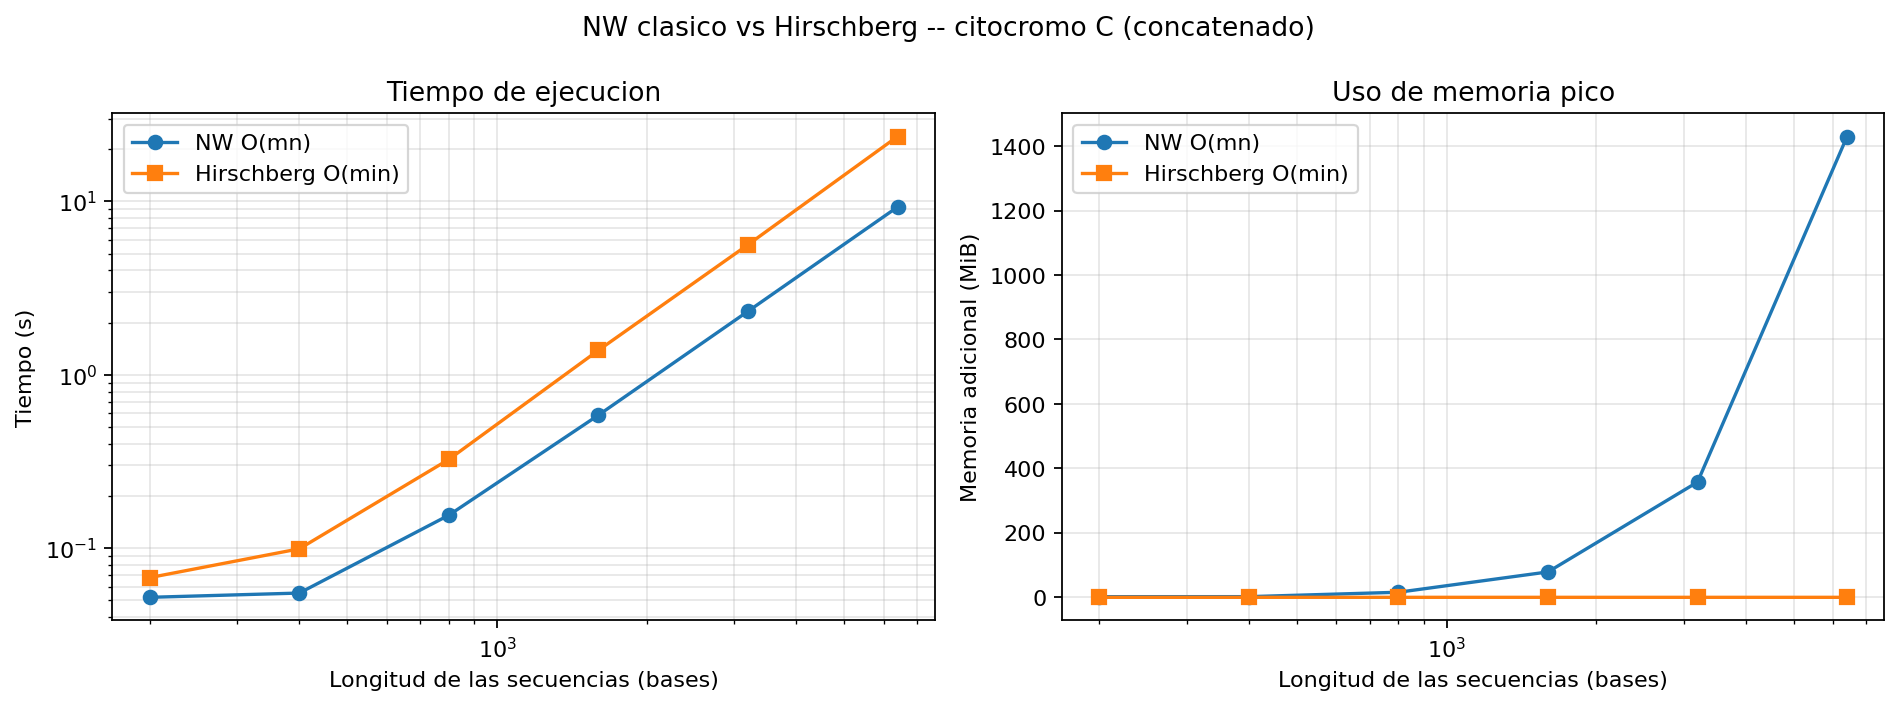
\includegraphics[width=\linewidth]{benchmark.png}
\end{columns}
\end{frame}

\begin{frame}{\textbf{Casos biol\'ogicos donde Hirschberg es cr\'itico}}
\begin{itemize}\setlength\itemsep{0.4em}
  \item \textbf{Transcritos largos.} mRNAs eucariotas $>$5~kb, alineamiento cDNA vs.\ genoma de referencia ($10^4$--$10^5$ bases).
  \item \textbf{M\'aquinas con memoria acotada.} Cl\'usters compartidos, contenedores Docker con l\'imites de RAM.
  \item \textbf{Mapeo de reads largos.} La idea de fondo de \texttt{minimap2} y \texttt{BWA}: \emph{nunca} materializar la matriz $O(mn)$.
\end{itemize}

\bigskip
\textbf{Mensaje:} la complejidad temporal $O(mn)$ es id\'entica entre ambas versiones; la diferencia es exclusivamente \textbf{memoria}. Para $mn$ grande, la memoria es el cuello de botella real.
\end{frame}

% ---------------------------------------------------------------
\section{Proyecto 2: filogenia del citocromo c}

\begin{frame}{Pipeline y datos}
\textbf{6 ort\'ologos de citocromo c} de UniProt (104--105 aa):
\smallskip
{\small\begin{tabular}{lll}
\toprule
Etiqueta & UniProt & Organismo \\
\midrule
Humano    & P99999 & \emph{Homo sapiens} \\
Chimpanc\'e & P99998 & \emph{Pan troglodytes} \\
Gorila    & G4XXM2 & \emph{Gorilla gorilla} \\
Rat\'on   & P62897 & \emph{Mus musculus} \\
Gallina   & P67881 & \emph{Gallus gallus} \\
At\'un    & P00025 & \emph{Katsuwonus pelamis} \\
\bottomrule
\end{tabular}}

\medskip
\textbf{Pipeline:}
\begin{enumerate}\setlength\itemsep{0.2em}
  \item NW + BLOSUM62, gap $-4$ sobre cada par $(i, j)$.
  \item Distancia $d_{ij} = 100 - \text{identidad}_{ij}$.
  \item Matriz $D \in \mathbb{R}^{6\times 6}$, sim\'etrica, $d_{ii}=0$.
  \item Dendrograma con UPGMA y single linkage (\texttt{scipy}, solo para dibujar).
\end{enumerate}
\end{frame}

\begin{frame}{Matriz de distancias 6$\times$6}
\centering
\begin{tabular}{lcccccc}
\toprule
            & Humano & Chimp & Gorila & Rat\'on & Gallina & At\'un \\
\midrule
Humano      & 0.0  & 0.0  & 0.0  & 8.6  & 12.4 & 20.0 \\
Chimpanc\'e & 0.0  & 0.0  & 0.0  & 8.6  & 12.4 & 20.0 \\
Gorila      & 0.0  & 0.0  & 0.0  & 8.6  & 12.4 & 20.0 \\
Rat\'on     & 8.6  & 8.6  & 8.6  & 0.0  & \alert{7.6}  & 15.2 \\
Gallina     & 12.4 & 12.4 & 12.4 & \alert{7.6}  & 0.0  & 16.2 \\
At\'un      & 20.0 & 20.0 & 20.0 & 15.2 & 16.2 & 0.0 \\
\bottomrule
\end{tabular}

\bigskip
\textbf{Observaciones:}
\begin{itemize}
  \item Primates entre s\'i: \textbf{identidad 100\,\%} (citocromo c maduro es id\'entico en los Hominidae, dato biol\'ogico real).
  \item Distancias monot\'onamente crecientes con la separaci\'on evolutiva.
  \item \alert{Anomal\'ia:} $d(\text{Rat\'on},\text{Gallina}) = 7.6 < d(\text{Humano},\text{Rat\'on}) = 8.6$.
\end{itemize}
\end{frame}

\begin{frame}{Validaci\'on contra Biopython (sustituto de BLAST)}
Los 15 pares fueron re-alineados con \texttt{Bio.Align.PairwiseAligner} (NW global, mismo BLOSUM62, mismo gap lineal $-4$).
\medskip

\textbf{Resultado: coincidencia exacta en score y \% identidad para los 15 pares.}

\smallskip
{\small\begin{tabular}{lcccc}
\toprule
Par & Score NW & \%id NW & Score Bio & \%id Bio \\
\midrule
Humano vs Chimpanc\'e & 565 & 100.0 & 565 & 100.0 \\
Humano vs Rat\'on     & 522 & 91.4  & 522 & 91.4  \\
Humano vs Gallina     & 507 & 87.6  & 507 & 87.6  \\
Humano vs At\'un      & 458 & 80.0  & 458 & 80.0  \\
Rat\'on vs Gallina    & 531 & 92.4  & 531 & 92.4  \\
Gallina vs At\'un     & 478 & 83.8  & 478 & 83.8  \\
\bottomrule
\end{tabular}}

\bigskip
$\Rightarrow$ Nuestra implementaci\'on de NW de la PC2 es \textbf{funcionalmente equivalente} a la est\'andar de Biopython para gap lineal.
\end{frame}

\begin{frame}{Dendrograma}
\centering
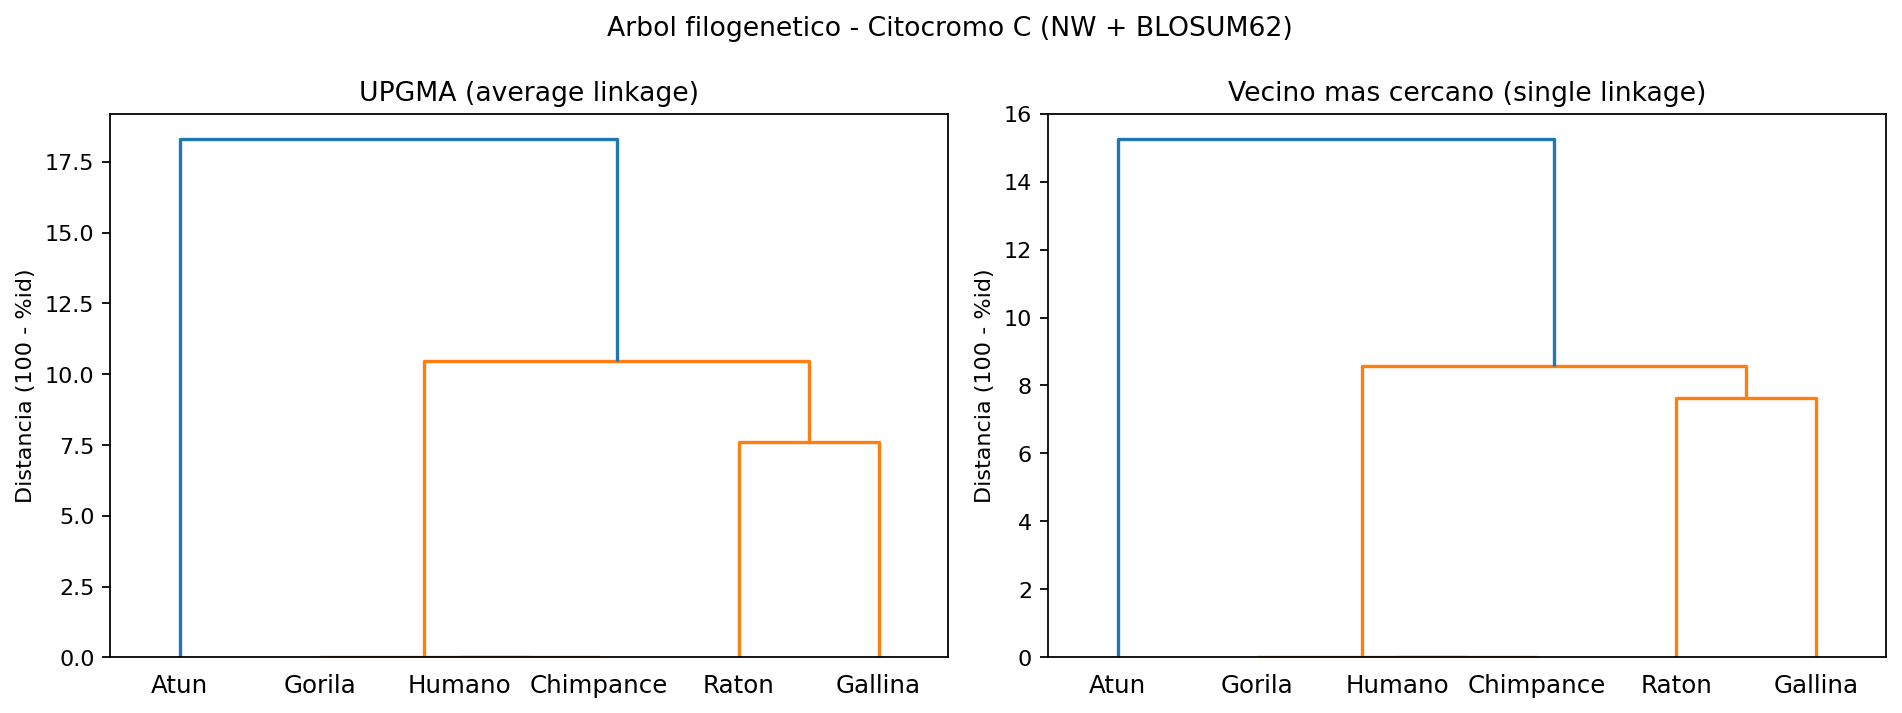
\includegraphics[width=\linewidth]{dendrogram.png}

\smallskip
\small UPGMA (izq.) y single linkage (der.). El clade primate colapsa a distancia 0; el at\'un es outgroup.
\end{frame}

\begin{frame}{\textbf{¿Coincide con el \'arbol evolutivo conocido?}}
\textbf{Topolog\'ia esperada:}
\[
\bigl(\bigl(\bigl((\text{Humano},\text{Chimp},\text{Gorila}),\text{Rat\'on}\bigr),\text{Gallina}\bigr),\text{At\'un}\bigr)
\]
Primates $\subset$ mam\'iferos $\subset$ amniotas $\subset$ vertebrados con mand\'ibula.

\bigskip
\textbf{Resultado: coincide \emph{parcialmente}.}
\begin{itemize}
  \item \alert{\checkmark} Primates agrupados correctamente (distancia 0 entre ellos).
  \item \alert{\checkmark} At\'un identificado correctamente como outgroup.
  \item \alert{$\boldsymbol{\times}$} La topolog\'ia interna falla: UPGMA agrupa (Rat\'on, Gallina) \emph{antes} que (Primates, Rat\'on), porque $d(\text{Rat\'on},\text{Gallina}) = 7.6 < d(\text{Humano},\text{Rat\'on}) = 8.6$.
\end{itemize}

\smallskip
\textbf{No es un bug del c\'odigo} (Biopython da exactamente las mismas distancias): es un problema del \emph{marcador molecular}.
\end{frame}

\begin{frame}{¿Por qu\'e falla el citocromo c?}
\begin{block}{1. Saturaci\'on del marcador}
Solo $\sim$30\% de las posiciones var\'ian. A divergencias $>$300~Ma (amniota/teleosteo), la mayor\'ia ya han mutado m\'ultiples veces $\to$ la identidad observada subestima la distancia real.
\end{block}
\begin{block}{2. Tasa heterog\'enea}
El linaje aviar (Gallina) evoluciona m\'as lento que el de los roedores (Dayhoff 1978) $\to$ Rat\'on--Gallina aparece artificialmente comprimido.
\end{block}
\begin{block}{3. Modelo de distancia ingenuo}
$d = 100(1-p)$ no corrige reversiones ni sustituciones m\'ultiples. Correcciones de Jukes--Cantor (ADN) o Poisson para prote\'inas ($d = -\ln p$) amplifican las distancias grandes y suelen corregir la paradoja.
\end{block}
\end{frame}

% ---------------------------------------------------------------
\section{Cierre}

\begin{frame}{Conclusiones}
\begin{enumerate}\setlength\itemsep{0.6em}
  \item \textbf{Hirschberg = score \'optimo de NW con memoria $O(\min(m,n))$.}
        Para 6400 bases: 1.4 GiB $\to$ 0 MiB adicionales, costo $\sim$2.5$\times$ en tiempo.
  \item \textbf{Filogenia con NW + BLOSUM62} reproduce el clade primate y el outgroup at\'un, pero falla en la topolog\'ia interna mam\'iferos/aves por saturaci\'on y heterogeneidad de tasa del citocromo c.
  \item \textbf{Validaci\'on:} 15/15 pares coinciden en score y \% identidad contra \texttt{Bio.Align.PairwiseAligner}.
  \item \textbf{Lectura central:} cambiar el \emph{algoritmo} (NW $\to$ Hirschberg) no altera la respuesta biol\'ogica; cambiar el \emph{marcador} s\'i. El algoritmo asegura optimalidad respecto a una funci\'on objetivo; la interpretaci\'on biol\'ogica depende del marcador, la matriz y el modelo de distancia.
\end{enumerate}
\end{frame}

\begin{frame}[standout]
Gracias.

\bigskip\small
\texttt{github.com/franklinep/-CC0F3-Biologia\_Computacional}
\end{frame}

\end{document}
